\documentclass[border=4mm]{standalone}
\usepackage{tikz}
\usepackage{amsmath}
\usepackage{mathptmx}
\usetikzlibrary{calc}

\begin{document}
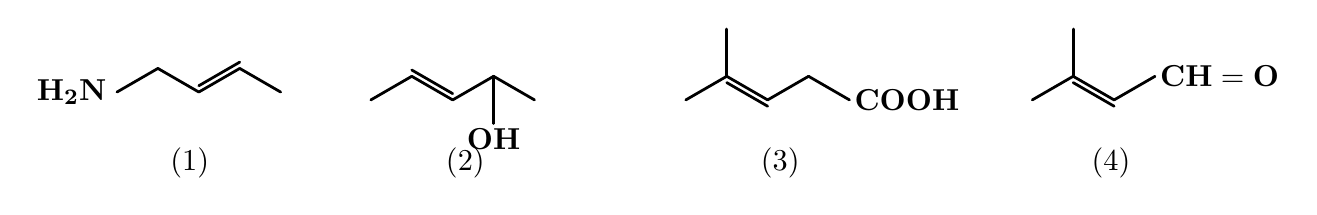
\begin{tikzpicture}[line cap=round, line join=round, line width=1.0pt, font=\fontsize{11}{13}\selectfont]
    % (1) H2N-CH2-CH=CH-CH3
    \begin{scope}[shift={(0,0)}]
        \node (N1) at (0,0) {$\mathbf{H_2N}$};
        \draw (N1.east) -- ++(30:0.6) -- ++(-30:0.6) coordinate (m1);
        % Nối đôi
        \draw (m1) -- ++(30:0.6) coordinate (m2);
        \draw ($(m1)+(0,0.08)$) -- ($(m2)+(0,0.08)$);
        \draw (m2) -- ++(-30:0.6);
        \node at (1.5,-0.9) {(1)};
    \end{scope}

    % (2) CH3-CH=CH-CH(OH)-CH3
    \begin{scope}[shift={(3.8,0)}]
        \coordinate (p0) at (0,-0.1);
        \draw (p0) -- ++(30:0.6) coordinate (p1);
        % Nối đôi
        \draw (p1) -- ++(-30:0.6) coordinate (p2);
        \draw ($(p1)+(0,0.08)$) -- ($(p2)+(0,0.08)$);
        % Nối tiếp
        \draw (p2) -- ++(30:0.6) coordinate (p3);
        \draw (p3) -- ++(-30:0.6);
        % Nhóm OH ở p3
        \draw (p3) -- ++(0,-0.6) node[below=-2pt] {$\mathbf{OH}$};
        \node at (1.2,-0.9) {(2)};
    \end{scope}

    % (3) CH3-C(CH3)=CH-CH2-COOH
    \begin{scope}[shift={(7.8,0)}]
        \coordinate (q0) at (0,-0.1);
        \draw (q0) -- ++(30:0.6) coordinate (q1);
        % Nhánh methyl hướng lên
        \draw (q1) -- ++(0,0.6);
        % Nối đôi
        \draw (q1) -- ++(-30:0.6) coordinate (q2);
        \draw ($(q1)+(0,-0.08)$) -- ($(q2)+(0,-0.08)$);
        % Nối tiếp CH2-COOH
        \draw (q2) -- ++(30:0.6) coordinate (q3);
        \draw (q3) -- ++(-30:0.6) node[right=-2pt] {$\mathbf{COOH}$};
        \node at (1.2,-0.9) {(3)};
    \end{scope}

    % (4) CH3-C(CH3)=CH-CH=O
    \begin{scope}[shift={(12.2,0)}]
        \coordinate (w0) at (0,-0.1);
        \draw (w0) -- ++(30:0.6) coordinate (w1);
        % Nhánh methyl hướng lên
        \draw (w1) -- ++(0,0.6);
        % Nối đôi
        \draw (w1) -- ++(-30:0.6) coordinate (w2);
        \draw ($(w1)+(0,-0.08)$) -- ($(w2)+(0,-0.08)$);
        % Nối tiếp CH=O
        \draw (w2) -- ++(30:0.6) node[right=-2pt] {$\mathbf{CH=O}$};
        \node at (1.0,-0.9) {(4)};
    \end{scope}
\end{tikzpicture}
\end{document}
